\documentclass{standalone}
\usepackage{tikz,pgf}

\begin{document}

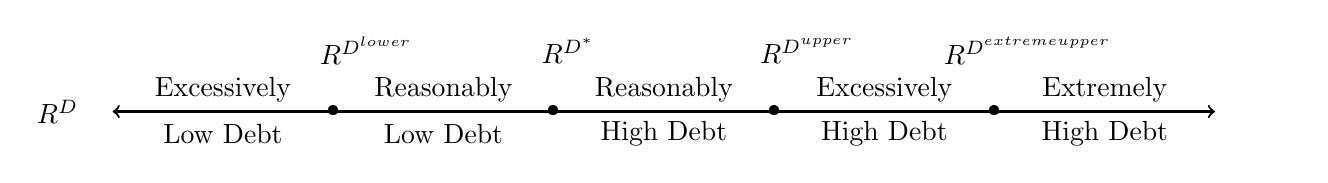
\begin{tikzpicture}[xscale=5.6,yscale=7]

\node [draw=none] at (1.75,0.04) {Extremely};
\node [draw=none] at (1.75,-0.04) {High Debt};

\node [draw=none] at (1.25,0.04) {Excessively};
\node [draw=none] at (1.25,-0.04) {High Debt};

\node [draw=none] at (0.75,0.04) {Reasonably};
\node [draw=none] at (0.75,-0.04) {High Debt};

\node [draw=none] at (0.25,0.04) {Reasonably};
\node [draw=none] at (0.25,-0.04) {Low Debt};

\node [draw=none] at (-0.25,0.04) {Excessively};
\node [draw=none] at (-0.25,-0.04) {Low Debt};

\node [draw=none] at (0.075,0.11) {$R^{D^{\text{lower}}}$};
\node [draw=none] at (0.533,0.11) {$R^{D^{*}}$};
\node [draw=none] at (1.075,0.11) {$R^{D^{\text{upper}}}$};
\node [draw=none] at (1.575,0.11) {$R^{D^{\text{extreme upper}}}$};

\foreach \Point in {0, 0.5, 1, 1.5}{
    \node[label={[label distance=1mm]:\rotatebox{0}{}}] at (\Point,0) {\textbullet};
}
\draw[thick,<->,color=black] (-0.5,0) -- (2,0); % Draw line
\node [draw=none] at (-0.625,0) {\bm{$R^D$}}; % Chart label
\node [draw=none] at (2.125,0)  {\color{white} $R_D$}; % Added to center chart

\end{tikzpicture}

\end{document}
